%++++++++++++++++++++++++++++++++++++++++
% Don't modify this section unless you know what you're doing!
\documentclass[letterpaper,12pt, reqno]{article}
\usepackage[utf8]{inputenc}
\usepackage[russian]{babel}
\usepackage{tikz}
\usepackage{graphicx}
\graphicspath{ {./images/} }
\usetikzlibrary{shapes.geometric,shapes.symbols,positioning,decorations.pathmorphing}
\usepackage{ amssymb }
\newcommand*\circled[1]{\tikz[baseline=(char.base)]{
            \node[shape=circle,draw,inner sep=2pt] (char) {#1};}}
\usepackage{tabularx} % extra features for tabular environment
\usepackage{amsmath}  % improve math presentation
\DeclareMathOperator*{\argmax}{argmax} % thin space, limits underneath in displays
\DeclareMathOperator*{\argmin}{argmin} % thin space, limits underneath in displays
\DeclareMathOperator*{\E}{\mathbb{E}}
\usepackage{graphicx} % takes care of graphic including machinery
\usepackage[margin=1in,letterpaper]{geometry} % decreases margins
\usepackage{cite} % takes care of citations
\usepackage[final]{hyperref} % adds hyper links inside the generated pdf file
\hypersetup{
	colorlinks=true,       % false: boxed links; true: colored links
	linkcolor=blue,        % color of internal links
	citecolor=blue,        % color of links to bibliography
	filecolor=magenta,     % color of file links
	urlcolor=blue         
}
%++++++++++++++++++++++++++++++++++++++++


\begin{document}

\title{Выпуская квалификационная работа}
\title{Свойства свёртки Гермейера в векторных играх }
\author{Кононов Сергей}
\date{\today}
\maketitle

\clearpage
\tableofcontents
\clearpage


\section{Введение}
\begin{flushleft}

Рассмотрим задачу многокритериальной или векторной, оптимизации:
\begin{equation}
\textrm{Найти }\max\limits_x F(x), \textrm{ где } F(x)=({f}_1(x),\ldots, {f}_n(x)),\quad x\in X\textrm{ конечно}
\end{equation}


\textbf{Определение [1]} 

Допустимое решение $\hat{x}\in{X}$ называется \textit{строго эффективным (эффективным по Слейтеру)}, если не существует
$x\in{X}$ такого, что $f(x)>f(\hat{x})$ т.е. $f_k(x)>f_k(\hat{x})$ для всех $k=1,...,n$. Множетсво всех эффективных по
Слейтеру решений называается \textit{множеством Слейтера} задачи (1).
\vspace{5mm}

Для параметризации задачи и поиска множества Слейтера используется метод свёрток, согласно которому МК-задача
$\max\limits_x F(x)$ заменяется параметрическим семейством скалярных задач $\max\limits_x C(\{f_i\}, \lambda)(x)$
где $C$ – функция свертки частных критериев $\{f_i\}_{i=1}^m$ МК-задачи в единый скалярный критерий (монотонна по f), 
$\lambda$ – параметр свертки. 
\vspace{5mm}

Мы рассмотрим \textit{линейную свёртку} (ЛС):
\begin{equation}
L(\{f_i\}, \lambda)(x)=\sum_{i=1}^{m} \lambda_i f_i \textrm{, где }
\lambda \in \Lambda =\{\lambda_i \geq 0 | \sum_{i=1}^n \lambda_i =1 \},
\end{equation}

и \textit{свёртку Гермейера}, или обратную логическую свёртку (ОЛС):
\begin{equation}
G(\{f_i\}, \lambda)(x)=\min\limits_{\lambda_i > 0} \frac{f_i}{\lambda_i} \textrm{, где }
\lambda \in \Lambda =\{\lambda_i \geq 0 | \sum_{i=1}^n \lambda_i =1 \}.
\end{equation}

\textbf{Игровая модель}

Студент (С) выбирает долю $x$ рабочего времени, которую он тратит на подготовку диплома. Допустим, что эффективность подготовки пропорциональна $\sqrt{x}$. Оставшееся рабочее время $1-x$ он тратит на подработку, и его второй 
критерий пропорционален $\sqrt{1-x}$. Считается, что производительность любых занятий С падает с увеличением отводимого на них времени, обусловливая вогнутость по $x$ частных критериев. Допустим, что Студент не может распределять свое время между двумя 
видами деятельности, т.е. имеет множетсво стратегий $x\in X = \{0, 1\}$, причём может использовать смешанные стратегии.
Преподаватель (П) имеет множество стратегий $y \in Y=\{1, 2\}$, причём тоже может использовать смешаные стратегии.
При этом П стремится минимизировать, а С максимизировать следующий векторный критерий: 
\begin{equation}
F(x, y)=(f_1(x, y), f_2(x, y)) =(\frac{y \sqrt{x}}{2}, \frac{\sqrt{1-x}}{y})
\end{equation}
Для введём обозначения для вероятностей:
\[
\begin{cases}
P(X=0)=1-q \\
P(X=1)=q \\
\end{cases}
\textrm{и }
\begin{cases}
P(Y=1)=1-p \\
P(Y=2)=p \\
\end{cases}
\]
И укажем области определения переменных, используемых ниже:
\[
p \in [0, 1],\quad q \in [0, 1],\quad
\mu \in [0, 1],\quad \lambda \in [0, 1]
\]

И предположим, что Студент осредняет свой критерий по переменной $x$ и получает:
$$F(q, y)=(f_1(q, y), f_2(q, y)) =\big(\frac{q y}{2}, \frac{1-q}{y}\big),$$
а Преподователь осредняет свой критерий по переменной $y$ и получает
$$F(x, p)=(f_1(x, p), f_2(x, p)) =\big(\frac{(1+p)\sqrt{x}}{2}, \frac{(2-p)\sqrt{1-x}}{2}\big)$$

\vspace{5mm}

Рассмотрим вариант, когда Студент использует обратную логическую свёртку и осредняет её по переменной $y$:
\begin{equation} 
M(p,q,\mu)=p\min{\{\frac{q}{\mu};\frac{1-q}{2(1-\mu)}\}}+(1-p)\min\{\frac{q}{2\mu};\frac{1-q}{1-\mu}\},
\end{equation}

a Преподаватель использует линейную свёртку и осредняет её по переменной $x$:
\begin{equation} 
L(p,q,\lambda)=\frac{1}{2}\big \{q(3\lambda+p-2)+(2-p)(1-\lambda)\big \}.
\end{equation} 

Игроки пытаются максимизировать или минимизировать сответствующие функции с помощью выбора своей стратегии
\[
\begin{cases} M(p,q,\mu)\rightarrow\max\limits_{q} \\
L(p,q,\lambda)\rightarrow\min\limits_{p}\end{cases}
\]
\textbf{Определение}

Пара стратегий $(p^{*}, q^{*})$ называется \textit{оптимальной}, если для некоторых $\lambda$, $\mu$ верно:
\begin{equation}
\begin{cases} 
p^{*}=p^{*}(q^{*}, \lambda) = \argmin\limits_{p} L(p, q^{*}, \lambda) \\ 
q^{*}=q^{*}(p^{*}, \mu) = \argmin\limits_{q} M(p^{*}, q, \mu) \\
\end{cases}
\end{equation}
\vspace{5mm}

Для исследования оптимальных стратегий необходимо установить значения $p$ и $q$, при которых
эти функции достигают минимума и максимума соответственно. Этот вопрос уже был исследован. Из статьи [3] следует, что:
\begin{equation}
p^{*}(q, \lambda)=\argmin\limits_{p}L(p,q,\lambda)=\begin{cases}0,& q>1-\lambda \\
1,& q<1-\lambda \\
\forall,& q=1-\lambda\end{cases}
\end{equation}

Из курсовой [2] следует, что
\begin{equation}
q^{*}(p, \mu)=\argmax\limits_{q}M(p,q,\mu)=
\begin{cases}
\frac{\mu}{2-\mu},& p+\mu-1\geq 0 \\
\frac{2\mu}{1+\mu},& p+\mu-1\leq 0 \\
\end{cases}
\end{equation}

%\section{Оптимальные стратегии}

%Для игрока П, использующего у = 2 с вероятностью р и ОЛС с параметром $\nu$, значение ОЛС и ее среднее дают формулы
%$$ M_{п}(x, p,\nu)=max\big\{ \frac{p\sqrt{x}+(1-p)\frac{\sqrt{x}}{2}}{\nu},\big\}$$

\section{Множество оптимальных стратегий}

\textbf{Утверждение}

Любая пара $(p^{*}, q^{*}) \in [0, 1]^{2}$ является оптимальной, т.е.  
$\forall$ $(p^{*}, q^{*}) \in [0, 1]^{2} \quad \exists$ $\mu, \lambda$: верно (7).
\vspace{5mm}

\textbf{Доказательство}

Зафиксируем некоторую пару  $(p^{*}, q^{*}) \in [0, 1]^{2}$ и найдя соответсвующие $\hat{\mu}(p^{*}, q^{*})$
 и $\hat{\lambda}(p^{*}, q^{*})$ покажем, что она является оптимальной.

\circled{1} Покажем оптимальность $p^{*}$:

Возьмём $\hat{\lambda}:=1-q^{*} \quad \Rightarrow$  поскольку 
$\argmin\limits_{p}L(p,q^{*},\hat{\lambda})=\forall$ при $ q^{*}=1-\hat{\lambda}$,

то и $p^{*} \in \argmin\limits_{p} L(p,q^{*},\hat{\lambda})$


\circled{2} Покажем оптимальность $q^{*}$:
\end{flushleft}
\center
\begin{tikzpicture}[scale=3]

% horizontal axis
\draw[->] (0,0) -- (1.2,0) node[anchor=north] {$\mu$};
% labels
\draw	(0,0) node[anchor=north] {0}
		(1,0) node[anchor=north] {1}
		(0, 1) node[anchor=east] {1}
		(0, 0.5) node[anchor=east] {$q^{*}$}
		(0.33, 0) node[anchor=north] {$\mu_2$}
		(0.66, 0) node[anchor=north] {$\mu_1$};

% ranges
\draw	(0.9,0.6) node{{\scriptsize $\frac{\mu}{2-\mu}$}}
		(0.6,0.9) node{{\scriptsize $\frac{2\mu}{1+\mu}$}};

% vertical axis
\draw[->] (0,0) -- (0,1.2) node[anchor=east] {$q$};
% nominal speed
\draw[dotted] (1,0) -- (1,1) -- (0, 1);
\draw[dotted] (0,0.5) -- (0.66,0.5) -- (0.66, 0);
\draw[dotted] (0.33,0) -- (0.33,0.5);

% Psis
\draw[domain=-0.1:1.1] plot({\x}, {\x / (2 - \x)});
\draw[domain=-0.1:1.1] plot({\x}, {2 * \x / (1 + \x)});

\end{tikzpicture}
\begin{flushleft}

По имеющемуся $q^{*}$ решим уравнения $f_1(\mu_1)=q^{*}$ и $f_2(\mu_2)=q^{*}$, где
$f_1=\frac{\mu}{2-\mu}$ и $f_2=\frac{2\mu}{1+\mu}$:

$$q^{*}=\frac{2\mu_2}{1+\mu_2} \Rightarrow \mu_2=\frac{q^{*}}{2-q^{*}}$$

$$q^{*}=\frac{\mu_1}{2-\mu_1} \Rightarrow \mu_1=\frac{2q^{*}}{1+q^{*}}$$
Заметим, что при $q^{*} \in [0, 1] \quad \mu_2 \leq \mu_1$ 

В таком случае поскольку $1-p^{*} \in [0, 1]$, то при фиксированных переменных 
$(p^{*}, q^{*})$ будет реализован один и только один из 3-х вариантов:

1) $1-p^{*} \leq \mu_2$
  
2) $\mu_2 < 1-p^{*} \leq \mu_1$

3) $\mu_1 < 1-p^{*}$
\vspace{5mm}

1) $1-p^{*} \leq \mu_2$, т.е.  $1-p^{*} \leq \frac{q^{*}}{2-q^{*}}$, в таком случае
$\hat{\mu}:=\mu_1=\frac{2q^{*}}{1+q^{*}}$.

Действительно, при таком выборе $\hat{\mu}$ имеем:  $1-p^{*} \leq \mu_2 \leq \mu_1 = \hat{\mu} \Rightarrow$
$p^{*}+\hat{\mu}-1 \geq 0 \Rightarrow \argmax\limits_{q}M(p^{*},q,\hat{\mu})=
\frac{\hat{\mu}}{2-\hat{\mu}}=\frac{\mu_1}{2-\mu_1}$=
$\frac{\frac{2q^{*}}{1+q^{*}}}{2-\frac{2q^{*}}{1+q^{*}}}=q^{*} \Rightarrow$ 
\[
\textrm{при}
\begin{cases}
\hat{\mu}=\frac{2q^{*}}{1+q^{*}} \\
\hat{\lambda} = 1 - q^{*} \\
1-p^{*} \leq \frac{q^{*}}{2-q^{*}}
\end{cases}
(p^{*}, q^{*}) - \textrm{оптимальная пара}
\] 

2) $\mu_2 < 1-p^{*} \leq \mu_1$, т.е.  $\frac{q^{*}}{2-q^{*}} < 1-p^{*} \leq \frac{2q^{*}}{1+q^{*}}$,
в таком случае $\hat{\mu}:=\mu_1=\frac{2q^{*}}{1+q^{*}}$.
Действительно, при таком выборе $\hat{\mu}$ имеем :$1-p^{*} \leq \mu_1 = \hat{\mu} \Rightarrow$
$p^{*}+\hat{\mu}-1 \geq 0 \Rightarrow \argmax\limits_{q}M(p^{*},q,\hat{\mu})=
\frac{\hat{\mu}}{2-\hat{\mu}}=\frac{\mu_1}{2-\mu_1}$=
$\frac{\frac{2q^{*}}{1+q^{*}}}{2-\frac{2q^{*}}{1+q^{*}}}=q^{*} \Rightarrow$ 

\[\
%\\textrm{при}\\\\
\begin{cases}
\hat{\mu}=\frac{2q^{*}}{1+q^{*}} \\
\hat{\lambda} = 1 - q^{*} \\
\frac{q^{*}}{2-1^{*}} < 1-p^{*} \leq \frac{2q^{*}}{1+q^{*}}
\end{cases}
(p^{*}, q^{*}) - \textrm{оптимальная пара}
\] 

3) $\mu_1 \leq 1-p^{*}$ т.е. $\frac{2q^{*}}{1+q^{*}} < 1-p^{*}$
в таком случае $\hat{\mu}=\mu_2=\frac{q^{*}}{2-q^{*}}$ 

действительно, при таком выборе $\hat{\mu}$ имеем $1-p^{*} \geq \mu_2 = \hat\mu \Rightarrow$
$p^{*}+\mu-1 \leq 0 \Rightarrow \argmax\limits_{q}M(p^{*},q,\hat{\mu})=
\frac{2\hat\mu}{1+\hat\mu}=\frac{2\mu_2}{1+\mu_2}=\frac{2\frac{q^{*}}{2-q^{*}}}{1+\frac{q^{*}}{2-q^{*}}}=
q^{*} \Rightarrow$ 
\[
\textrm{при}
\begin{cases}
\hat\mu=\frac{q^{*}}{2-q^{*}} \\
\hat\lambda = 1 - q^{*} \\
\frac{2q^{*}}{1+q^{*}} < 1-p^{*}
\end{cases}
(p^{*}, q^{*}) - \textrm{оптимальная пара}
\] 

Таким образом при имеющихся $(p^{*},q^{*})$ сначала надо определить в какой из вариантов 1-3 пара попадает, затем
по соответсвующим равенствам найти $\hat\mu$ и $\hat\lambda$.

\textbf{Утверждение доказано.}

\section{Графическое изображение матожидания критерия}
Вычислим матожидание от имеющегося векторного критерия для игрока П
$F(X, Y) = \big(\frac{Y\sqrt{X}}{2};\frac{\sqrt{1-X}}{Y}\big)$, где $X$ и $Y$ - случайные величины, причём
\[
\begin{cases}
P(X=0)=1-q \\
P(X=1)=q \\
\end{cases}
\begin{cases}
P(Y=1)=1-p \\
P(Y=2)=p \\
\end{cases}
\]

В таком случае имеем:
\begin{equation}
\E_{x} [F(x,y)]=\big(\frac{yq}{2};\frac{1-q}{y}\big)
\end{equation}
\begin{equation}
\E_{xy} [F(x,y)]=\big(\frac{q(1+p)}{2};\frac{(1-q)(2-p)}{2}\big)
\end{equation}

Рассмотрим это как множество точек на плоскости $X,Y$ зависящие от двух параметров $(p,q)\in[0,1]^2$
\[
\begin{cases}
y=\frac{q(1+p)}{2} \\
x=\frac{(1-q)(2-p)}{2}  
\end{cases}
\Rightarrow
\begin{cases}
q=\frac{2x}{1+p} \\
y=(1-\frac{2x}{1+p})\frac{2-p}{2}=\frac{(1+p-2x)(2-p)}{2(1+p)}
\end{cases}
\]

Найдём максимальные значения, которые может принимать $y(x, p)$ при фиксированном $x$:
$$
\frac{\partial{y(x,p)}}{\partial{p}}=\frac{3x}{(p+1)^2} - \frac{1}{2}=0 
\Rightarrow
p_0=\sqrt{6x} - 1
$$
Поскольку область определения $p_0\in[0, 1]$, и 
$$
p_0 = 1 \Rightarrow x=\frac{2}{3} \textsl{ и }
p_0 = 0 \Rightarrow x=\frac{1}{6}
$$
 
$$y_{max}(x) = 
\begin{cases}
\max(y(x, 0), y(x, 1), y(x, p_0)), & x\in[\frac{1}{6}, \frac{2}{3}] \\
\max(y(x, 0), y(x, 1)), & x\in[0, \frac{1}{6}] \cap [\frac{2}{3}, 1]
\end{cases}
$$

учитывая, что 
$$y(x, 0) = 1 - 2x $$
$$y(x, 1) = \frac{1-x}{2}$$ 
$$y(x,p_0) = \frac{(\sqrt{6x} - 2x)(3-\sqrt{6x})}{2\sqrt{6x}}$$

$$y_{min}(x)=
\begin{cases}
\frac{1-x}{2}, &x\in[0,\frac{1}{3}] \\
1-2x, &x\in(\frac{1}{3},1]
\end{cases}
\quad
y_{max}(x)=
\begin{cases}
1-2x, &x\in[0,\frac{1}{6}] \\
\frac{(\sqrt{6x} - 2x)(3-\sqrt{6x})}{2\sqrt{6x}}, &x\in(\frac{1}{6},\frac{2}{3}]\\
\frac{1-x}{2}, &x\in(\frac{2}{3},1]
\end{cases}
$$

В предыдущем пункте мы установили что любая пара $(p^{*}, q^{*}) \in [0, 1]^{2}$ является оптимальной. Теперь для всех
оптимальных стратегий т.е. пар $(p^{*}, q^{*}) \in [0, 1]^{2}$ изобразим на графике значения матожидания векторного критерия в этой
точке.
\begin{center}
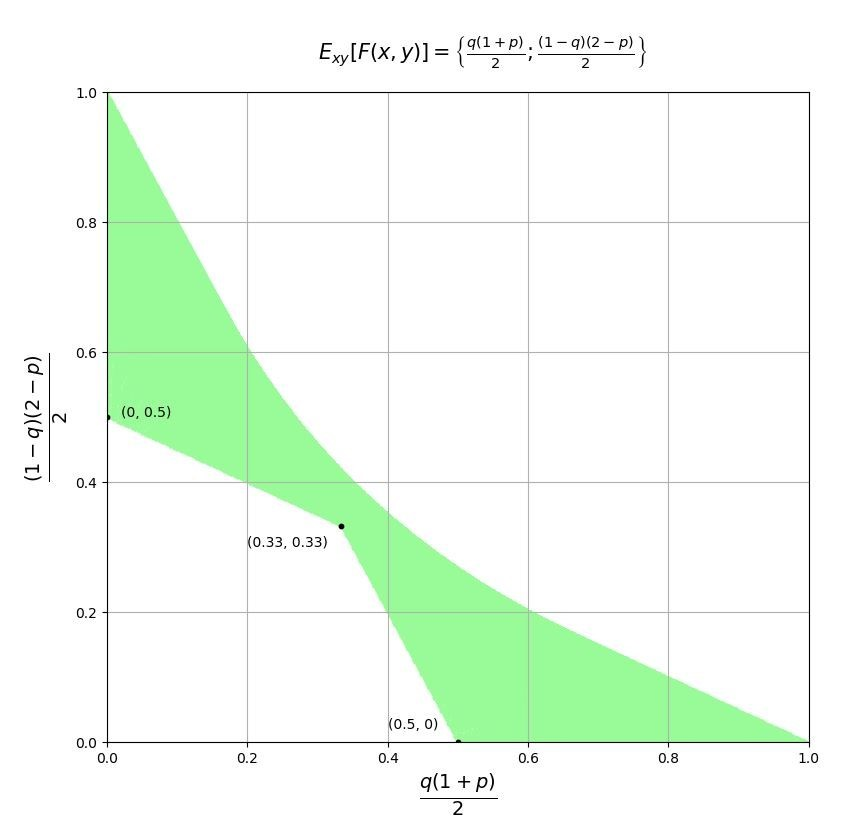
\includegraphics[scale=0.8]{graf_1_2}
\end{center}




\section{Оптимальные результаты для игрока С}

Теперь рассмотрим игру с точки зрения игрока С. Для каждой пары параметров $(\hat\mu, \hat\lambda)$ найдём
множество соответсвующих оптимальных пар $(p^*(\hat\mu, \hat\lambda), q^*(\hat\mu, \hat\lambda))$. Далее 
найдём значение свёртки для игрока С в этих точка:
$$
M(p^*,q^*,\hat\mu)=p^*\min{\{\frac{q^*}{\hat\mu};\frac{1-q^*}{2(1-\hat\mu)}\}} +
				   (1-p^*)\min\{\frac{q^*}{2\hat\mu};\frac{1-q^*}{1-\hat\mu}\}
$$
И изобразим множество значений функции в этих точках.
\vspace{5mm}
 
Рассмотрим все возможные сочетания значений для $p^{*}$ и $q^{*}$ в системах (7) и (8), что даст нам 6 следующих систем:
\vspace{5mm}

Напомню, что переменные имеют следующих области ограничений:
\[
p \in [0, 1],\quad q \in [0, 1],\quad
\mu \in [0, 1],\quad \lambda \in [0, 1]
\]
\circled{1}%---------------------------1------------------------
\[
\begin{cases}
p^{*}=0 \\
q^{*}=\frac{\mu}{2-\mu} \\
q^{*}>1-\lambda \\
p^{*}+\mu-1\geq 0 \\
\end{cases}
\quad\sim\quad
\begin{cases}
p^{*}=0 \\
q^{*}=\frac{\mu}{2-\mu} \\
\frac{\mu}{2-\mu}>1-\lambda \\
\mu\geq 1 \quad\Rightarrow\quad \mu=1 \\
\end{cases}
\quad\sim\quad
\begin{cases}
p^{*}=0 \\
q^{*}=1 \\
\lambda>0 \\
\mu=1
\end{cases}
\]
Значит при $\mu=1$, $\lambda\in(0,1]$ имеем следующие оптимальные пары
$\begin{cases}p^{*}=0 \\ q^{*}=1 \end{cases}$

\circled{2}%---------------------------2------------------------
\[
\begin{cases}
p^{*}=0 \\
q^{*}=\frac{2\mu}{1+\mu} \\
q^{*}>1-\lambda \\
p^{*}+\mu-1\leq 0 \\
\end{cases}
\quad\sim\quad
\begin{cases}
p^{*}=0 \\
q^{*}=\frac{2\mu}{1+\mu} \\
\frac{2\mu}{1+\mu}>1-\lambda \\
\mu \leq 1
\end{cases}
\quad\sim\quad
\begin{cases}
p^{*}=0 \\
q^{*}=\frac{2\mu}{1+\mu} \\
\lambda>\frac{1-\mu}{1+\mu} \\
\mu \leq 1
\end{cases}
\]
Значит при $\mu \in [0, 1]$, $\lambda \in (\frac{1-\mu}{1+\mu}, 1]$ имеем следующие оптимальные пары
$\begin{cases}p^{*}=0 \\ q^{*}=\frac{2\mu}{1+\mu} \end{cases}$



\circled{3}%---------------------------3------------------------
\[
\begin{cases}
p^{*}=1 \\
q^{*}=\frac{\mu}{2-\mu} \\
q^{*}<1-\lambda \\
p^{*}+\mu-1\geq 0 \\
\end{cases}
\quad\sim\quad
\begin{cases}
p^{*}=1 \\
q^{*}=\frac{\mu}{2-\mu} \\
\frac{\mu}{2-\mu}<1-\lambda \\
\mu \geq 0
\end{cases}
\quad\sim\quad
\begin{cases}
p^{*}=1 \\
q^{*}=\frac{\mu}{2-\mu} \\
\lambda<2\frac{1-\mu}{2-\mu} \\
\mu \geq 0
\end{cases}
\]
Значит при $\mu \in [0, 1]$, $\lambda \in [0, 2\frac{1-\mu}{2-\mu})$ имеем следующие оптимальные пары
$\begin{cases}p^{*}=1 \\ q^{*}=\frac{\mu}{2-\mu} \end{cases}$


\circled{4}%---------------------------4------------------------
\[
\begin{cases}
p^{*}=1 \\
q^{*}=\frac{2\mu}{1+\mu} \\
q^{*}<1-\lambda \\
p^{*}+\mu-1 \leq 0 \\
\end{cases}
\quad\sim\quad
\begin{cases}
p^{*}=1 \\
q^{*}=\frac{2\mu}{1+\mu} \\
\frac{2\mu}{1+\mu}<1-\lambda \\
\mu \leq 0 \quad\Rightarrow\quad \mu=0 \\
\end{cases}
\quad\sim\quad
\begin{cases}
p^{*}=1 \\
q^{*}=0 \\
\lambda<1 \\
\mu=0
\end{cases}
\]
Значит при $\mu=0$, $\lambda \in [0, 1)$ имеем следующие оптимальные пары
$\begin{cases}p^{*}=1 \\ q^{*}=0 \end{cases}$


\circled{5} %---------------------------5------------------------
\[
\begin{cases}
p^{*} \in [0, 1] \\
q^{*}=\frac{\mu}{2-\mu} \\
q^{*}=1-\lambda \\
p^{*}+\mu-1 \geq 0 \\
\end{cases}
\quad\sim\quad
\begin{cases}
p^{*} \in [0, 1] \\
q^{*}=\frac{\mu}{2-\mu} \\
\frac{\mu}{2-\mu}=1-\lambda \\
p^* \geq 1-\mu \\
\end{cases}
\quad\sim\quad
\begin{cases}
p^* \in [1-\mu, 1] \\
q^{*}=\frac{\mu}{2-\mu} \\
\lambda=2\frac{1-\mu}{2-\mu} \\
\end{cases}
\]
Значит при $\lambda=2\frac{1-\mu}{2-\mu}$, $\mu \in [0, 1]$ имеем следующие оптимальные пары
$\begin{cases}p^{*} \in [1-\mu, 1] \\ q^{*}=\frac{\mu}{2-\mu} \end{cases}$


\circled{6}%---------------------------6------------------------
\[
\begin{cases}
p^{*} \in [0, 1] \\
q^{*}=\frac{2\mu}{1+\mu} \\
q^{*}=1-\lambda \\
p^{*}+\mu-1 \leq 0 \\
\end{cases}
\quad\sim\quad
\begin{cases}
p^{*} \in [0, 1] \\
q^{*}=\frac{2\mu}{1+\mu} \\
\frac{2\mu}{1+\mu}=1-\lambda \\
p^{*} \leq 1 - \mu 
\end{cases}
\quad\sim\quad
\begin{cases}
p^{*} \in [0, 1-\mu] \\
q^{*}=\frac{2\mu}{1+\mu} \\
\lambda = \frac{1-\mu}{1+\mu} \\
\end{cases}
\]
Значит при $\mu \in [0, 1]$, $\lambda = \frac{1-\mu}{1+\mu} $ имеем следующие оптимальные пары
$\begin{cases}
p^{*} \in [0, 1-\mu] \\
q^{*}=\frac{2\mu}{1+\mu} \\
\end{cases}$
\vspace{10mm}

Теперь на квадрате $(p,q)\in[0, 1]^{2}$ рассмотрим все области, в которых множества оптимальных пар постоянны. И найдём множества значений функции 
\[
M(p,q,\mu)=p\min{\{\frac{q}{\mu};\frac{1-q}{2(1-\mu)}\}}+(1-p)\min\{\frac{q}{2\mu};\frac{1-q}{1-\mu}\}
\]
В этих областях

\begin{center}
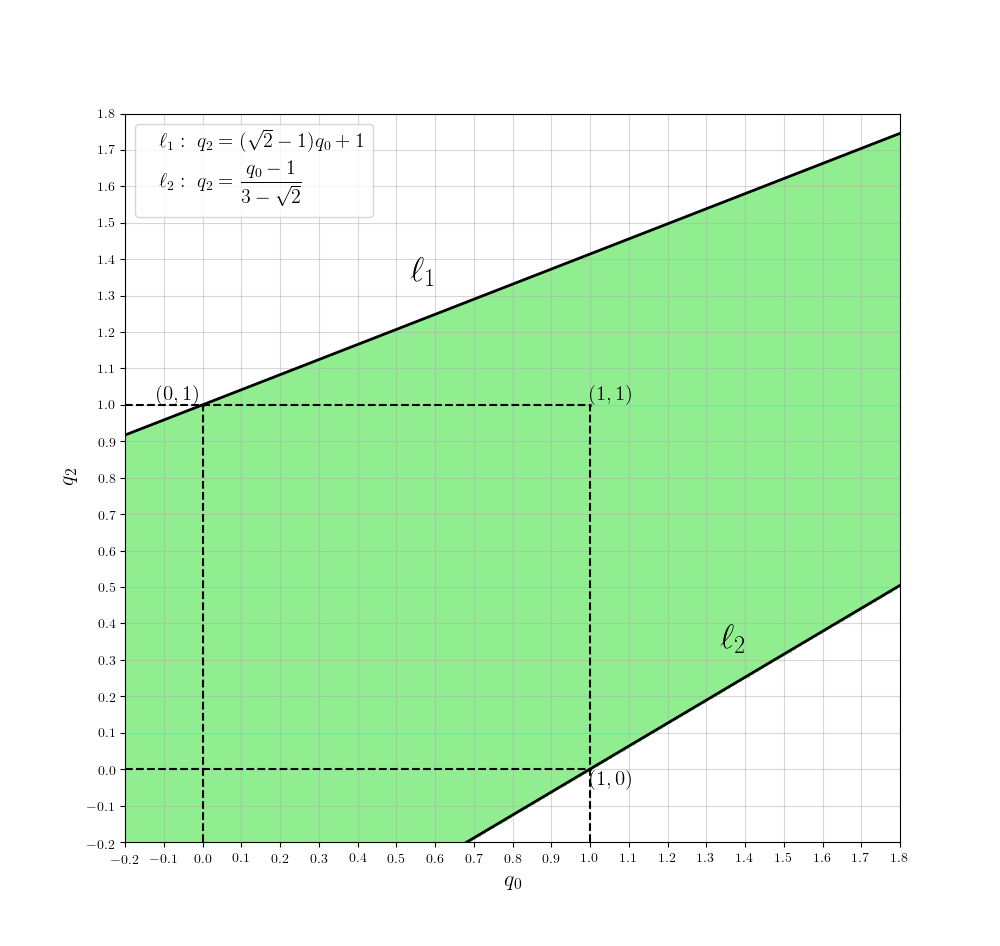
\includegraphics[scale=0.4]{graf_3_1}
\end{center}

1) $\mu=0$, $\lambda \in [0, 1)$: 
$\begin{cases}p^{*}=1 \\ q^{*}=0 \end{cases};
\begin{cases}p^{*}=1 \\ q^{*}=\frac{\mu}{2-\mu} 
= \{\mu=0\}=0 \end{cases} $ \hfill \break
Получаем множества оптимальных стратегий 
$(P^{*} \times Q^{*}) =(\{1\} \times \{0\})$, где $\times$ - это декартово произведение, тогда
$$M(1,0,0)=\frac{1}{2}$$


\begin{center}
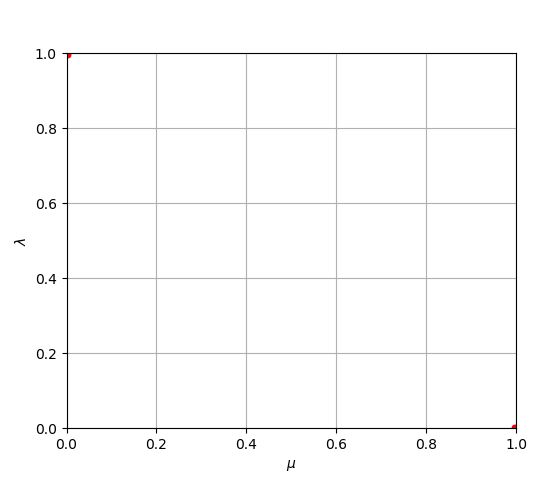
\includegraphics[scale=0.7]{graf_3_2}
\end{center}
2.1) $\mu=0$, $\lambda =1$: 
$\begin{cases}p^{*} \geq 1-\mu = \{\mu=0\}=1
\\ q^{*}=\frac{\mu}{2-\mu} = \{\mu=0\}=0
\end{cases}$;
$\begin{cases}p^{*} \leq 1-\mu = \{\mu=0\}=1\\\
q^{*}=\frac{2\mu}{1+\mu}= \{\mu=0\}=0 \end{cases}$
\hfill \break 
Получаем множества оптимальных стратегий 
$(P^{*} \times Q^{*}) =([0, 1] \times \{0\})$ тогда
$$M([0, 1],0,0)=[0.5,1]$$
%\vspace{5mm}

2.2) $\mu=1$, $\lambda=0$: 
$\begin{cases}p^{*} \geq 1-\mu = \{\mu=1\}=0
\\ q^{*}=\frac{\mu}{2-\mu} = \{\mu=1\}=1
\end{cases}$;
$\begin{cases}p^{*} \leq 1-\mu = \{\mu=1\}=0\\\
q^{*}=\frac{2\mu}{1+\mu}= \{\mu=1\}=1 \end{cases}$
\hfill \break 
Получаем множества оптимальных стратегий 
$(P^{*} \times Q^{*}) =([0, 1] \times \{1\})$ тогда
$$M([0, 1],1,1)=[0.5,1]$$
%\vspace{5mm}

\begin{center}
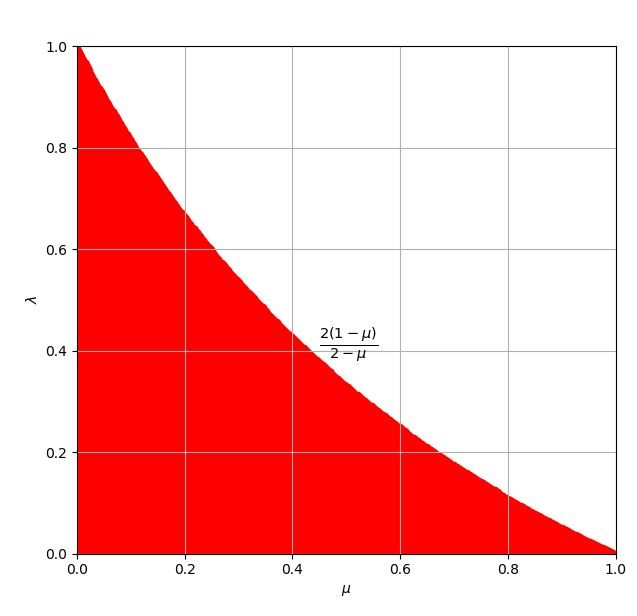
\includegraphics[scale=0.6]{graf_3_3}
\end{center}
3) $\mu \in (0,1)$, $\lambda\in(0,\frac{1-\mu}{1+\mu}]$: 
$\begin{cases}p^{*}=1 \\ q^{*}=\frac{\mu}{2-\mu} \end{cases}$
\hfill \break
Получаем множества оптимальных стратегий 
$(P^{*} \times Q^{*}) =(\{1\} \times \{\frac{\mu}{2-\mu}\})$ тогда
$$M(1,\frac{\mu}{2-\mu},\mu)=\min \big\{\frac{\mu}{2-\mu}; 
\frac{1-\frac{\mu}{2-\mu}}{2(1-\mu)}\big\}=\frac{1}{2-\mu}$$
%\vspace{5mm}

\begin{center}
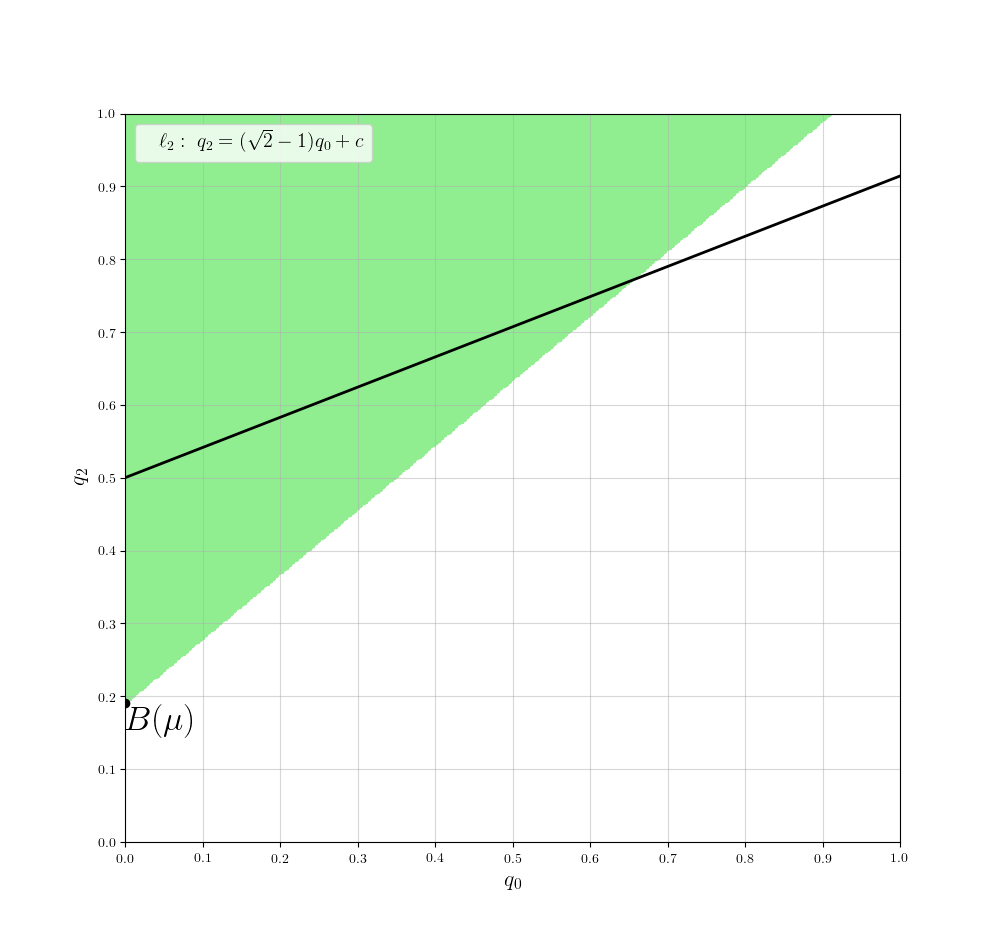
\includegraphics[scale=0.6]{graf_3_4}
\end{center}
4) $\mu \in (0,1)$, $\lambda=\frac{1-\mu}{1+\mu}$:
$\begin{cases}p^{*} \in [0, 1-\mu] \cup \{1\} \\
q^{*} = \frac{\mu}{2-\mu}
\end{cases}$
\hfill \break
4.1) Получаем множества оптимальных стратегий 
$(P^{*} \times Q^{*}) =(\{1\} \times \{\frac{\mu}{2-\mu}\})$ тогда
$$M(1,\frac{\mu}{2-\mu},\mu)=\frac{1}{2-\mu}$$

4.2) Получаем множества оптимальных стратегий 
$(P^{*} \times Q^{*}) =([0,1-\mu] \times \{\frac{2\mu}{1+\mu}\})$ тогда
$$M(p,\frac{2\mu}{1+\mu},\mu)=p\frac{1}{2(1+\mu)}+(1-p)\frac{1}{1+\mu}=\frac{2-p}{2(1+\mu)} \geq
\frac{2 - (1-\mu)}{2(1+\mu)}=\frac{1+\mu}{2(1+\mu)}=\frac{1}{2}$$
$$M(p,\frac{2\mu}{1+\mu},\mu) \leq \frac{1}{1+\mu} \Rightarrow M(p,\frac{2\mu}{1+\mu},\mu) = [0.5, \frac{1}{1+\mu}]$$

\begin{center}
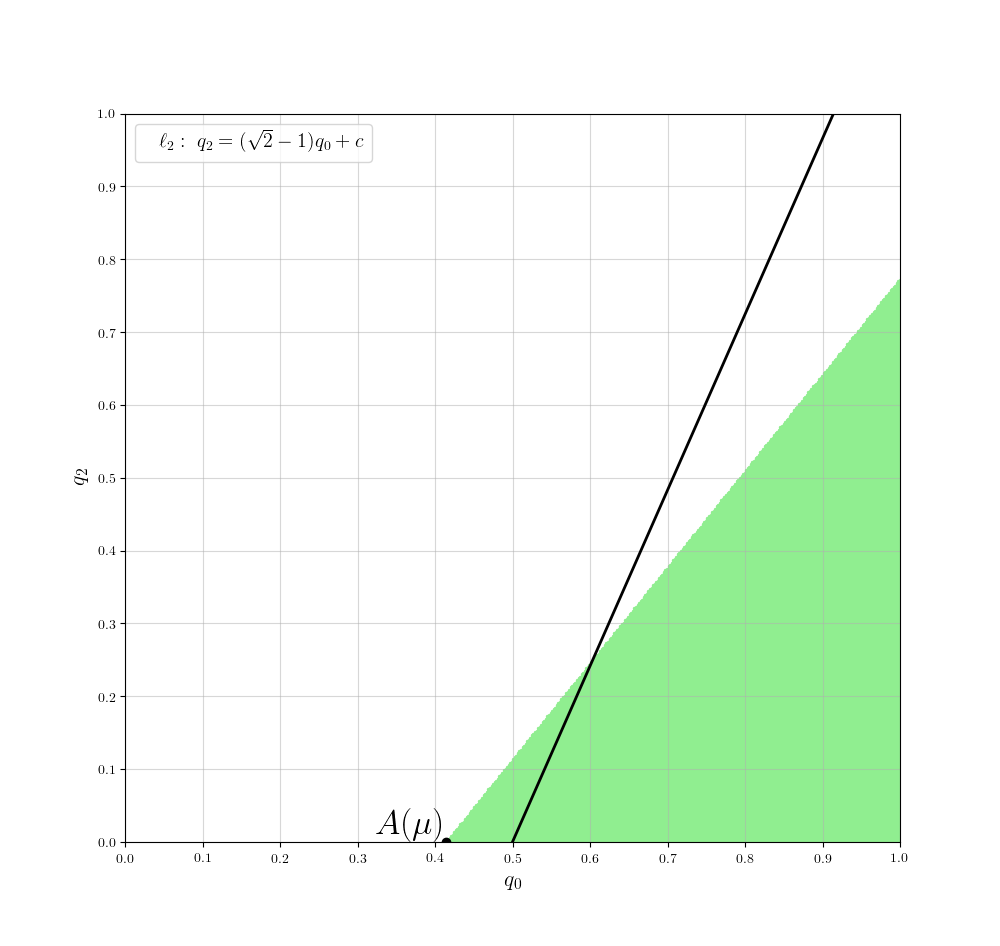
\includegraphics[scale=0.5]{graf_3_5}
\end{center}
5) $\mu \in [(, 1)$, $\lambda \in [0, 2\frac{1-\mu}{2-\mu}]\cap(\frac{1-\mu}{1+\mu}, 1]$: 
$\begin{cases}p^{*}=0 \\ q^{*}=\frac{2\mu}{1+\mu} \end{cases}$;
$\begin{cases}p^{*}=1 \\ q^{*}=\frac{\mu}{2-\mu} \end{cases}$
\hfill \break
5.1) Получаем множества оптимальных стратегий 
$(P^{*} \times Q^{*}) =(\{0\} \times \{\frac{2\mu}{1+\mu}\})$ тогда
$$M(0, \frac{2\mu}{1+\mu},\mu)=\frac{1}{1+\mu}$$
5.2) Получаем множества оптимальных стратегий 
$(P^{*} \times Q^{*}) =(\{1\}\times \{\frac{\mu}{2-\mu}\})$ тогда
$$M(1, \frac{\mu}{2-\mu},\mu)=\frac{1}{2-\mu}$$

\begin{center}
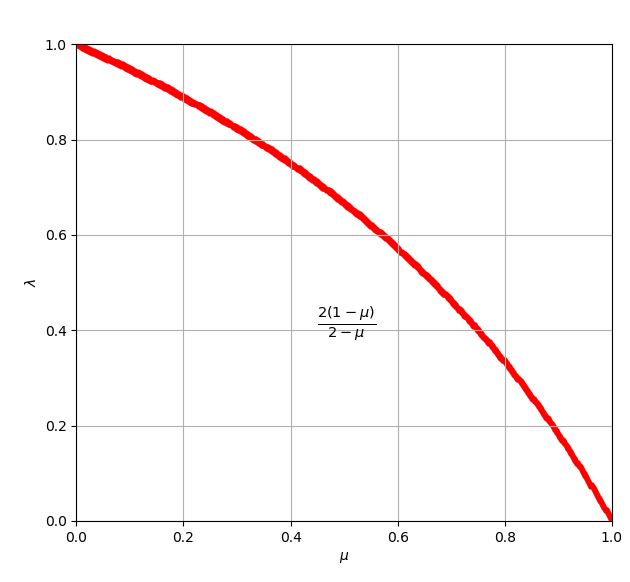
\includegraphics[scale=0.5]{graf_3_6}
\end{center}
6) $\mu \in (0, 1)$, $\lambda = 2\frac{1-\mu}{2-\mu}$: 
$\begin{cases}p^{*}=0 \\ q^{*}=\frac{2\mu}{1+\mu} \end{cases}$;
$\begin{cases}p^{*} \in [0,1-\mu] \\ q^{*}=\frac{\mu}{2-\mu} \end{cases}$
\hfill \break
6.1) Получаем множества оптимальных стратегий 
$(P^{*} \times Q^{*}) =(\{0\} \times \{\frac{2\mu}{1+\mu}\})$ тогда
$$M(0, \frac{2\mu}{1+\mu}, \mu)=\frac{1}{1+\mu}$$
6.2) Получаем множествo оптимальных стратегий 
$(P^{*}\times Q^{*}) =([1-\mu,1] \times \{\frac{\mu}{2-\mu}\})$ тогда
$$M(p,\frac{\mu}{2-\mu},\mu)=p\frac{1}{2-\mu}+(1-p)\frac{1}{2(2-\mu)}=\frac{1+p}{2(2-\mu)} \geq \frac{2-\mu}{2(2-\mu)}=\frac{1}{2}$$
$$M(p,\frac{\mu}{2-\mu},\mu) \leq \frac{1}{2-\mu} \Rightarrow M(p,\frac{\mu}{2-\mu},\mu) = [0.5, \frac{1}{2-\mu}]$$


\begin{center}
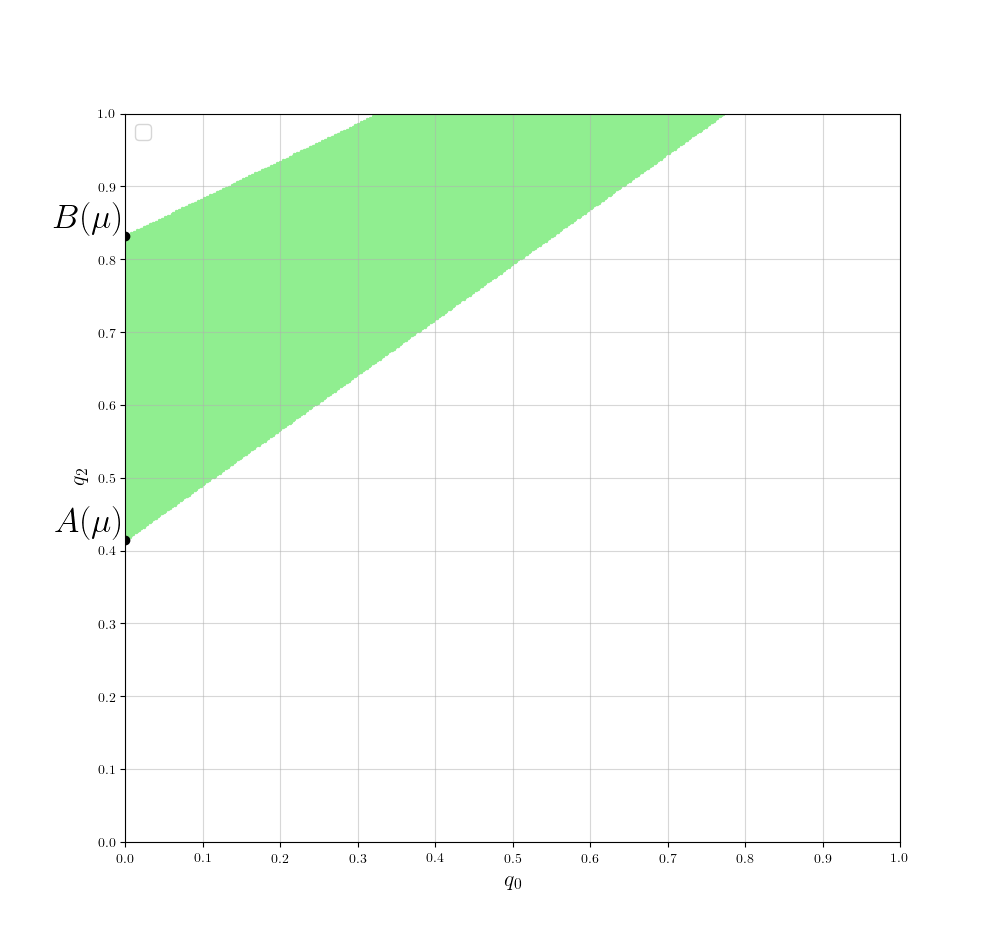
\includegraphics[scale=0.5]{graf_3_7}
\end{center}
7) $\mu \in (0, 1), \lambda \in (2\frac{1-\mu}{2-\mu}, 1]$: 
$\begin{cases}p^{*} =0 \\ q^{*}=\frac{2\mu}{1+\mu} \end{cases}$
\hfill \break
Получаем множества оптимальных стратегий 
$(P^{*} \times Q^{*}) =(\{0\} \times \{\frac{2\mu}{1+\mu}\})$ тогда
$$M(0, \frac{2\mu}{1+\mu}, \mu)=\min \big\{\frac{1}{\mu}\frac{2\mu}{1+\mu}; 
\frac{1-\frac{2\mu}{1+\mu}}{1-\mu}\big\}=\frac{1}{1+\mu}$$

\begin{center}
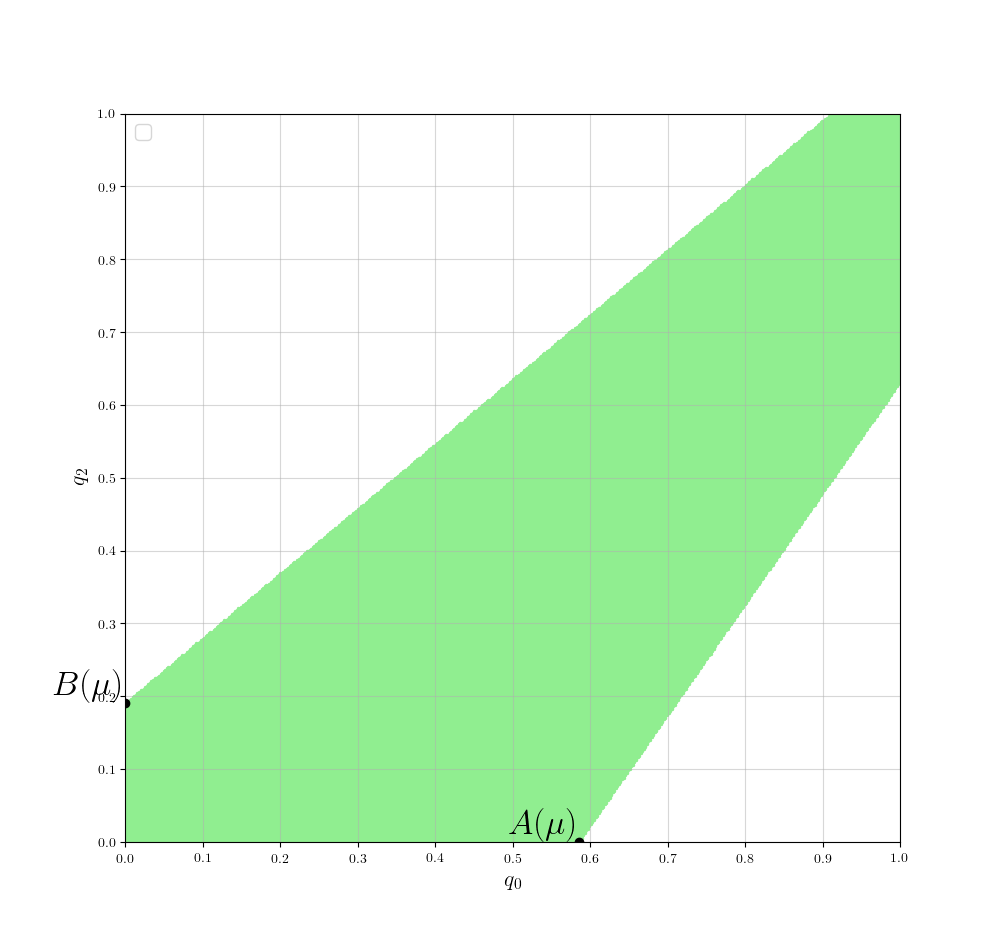
\includegraphics[scale=0.5]{graf_3_8}
\end{center}
8) $\mu = 1$, $\lambda \in (0, 1] $: 
$\begin{cases}
p^{*}=0 \\
q^{*}=1 \\
\end{cases}$;
$\begin{cases}
p^{*}=0 \\
q^{*}=\frac{2\mu}{1+\mu}=\{\mu=1\}=1 \\
\end{cases}$
\hfill \break
Получаем множества оптимальных стратегий 
$(P^{*} \times Q^{*}) =(\{0\} \times \{1\})$ тогда
$$M(0, 1, 1)=\frac{1}{2}$$
\vspace{40mm}

Теперь на квадрате $(\mu,\lambda)\in[0, 1]^{2}$ мы рассмотрели все точки и для каждой нашли оптимальные пары $p^{*}(\mu, \lambda)$
и $q^{*}(\mu, \lambda)$ и соответсвующие значения функции $M(p^{*}(\mu, \lambda),q^{*}(\mu, \lambda),\mu)$. Далее на квадрате
$[0, 1]^{2}$ изобразим все точки, которые принимает вектор $(\mu M(p^{*},q^{*},\mu), (1-\mu) M(p^{*},q^{*},\mu))$ при
$(\mu, \lambda)\in[0, 1]^{2}$

\begin{center}
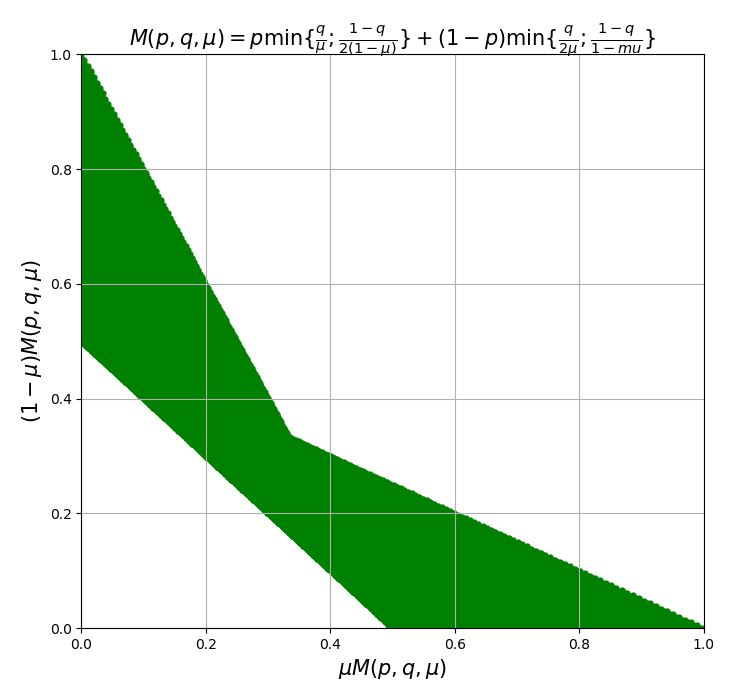
\includegraphics[scale=0.6]{graf_4}
\end{center}

Поясним график: \\
нижняя огибающая в координатах $X,Y$: $y=\frac{1}{2}-x$, \\
верхняя огибающая в координатах $X,Y$: $y=
\begin{cases}
1-2x, & x \in [0, \frac{1}{3}) \\
\frac{1-x}{2}, & x \in [\frac{1}{3}, 1]
\end{cases}.
$

\section{Заключение}
Итого мы выполнили поставленную задачу.

\section{Ссылки на источники}
[1] Matthais Ehrgott. \textit{Multicriterial optimization. page 38, Defenition 2.24}

[2] Н.М. Новикова, И.И. Поспелова. \textit{Смешанные стратегии в векторной оптимизациий и свёртка Гермейера.}

[3] С.В. Кононов. \textit{Смешанные стратегии в векторной оптимизации и свертка Гермейера.}

[4] Ю.Б. Гермейер \textit{Введение в теорию исслежования операций}


\end{flushleft}
\end{document}